\documentclass[a4paper]{report}
\usepackage[utf8]{inputenc}
\usepackage[german]{babel}
\usepackage{graphicx}
\usepackage[font]{}

\begin{document}

\chapter{Einführung}

Die  vier Wirtschaft Subjekten:
\newline
\newline
\newline
\newline
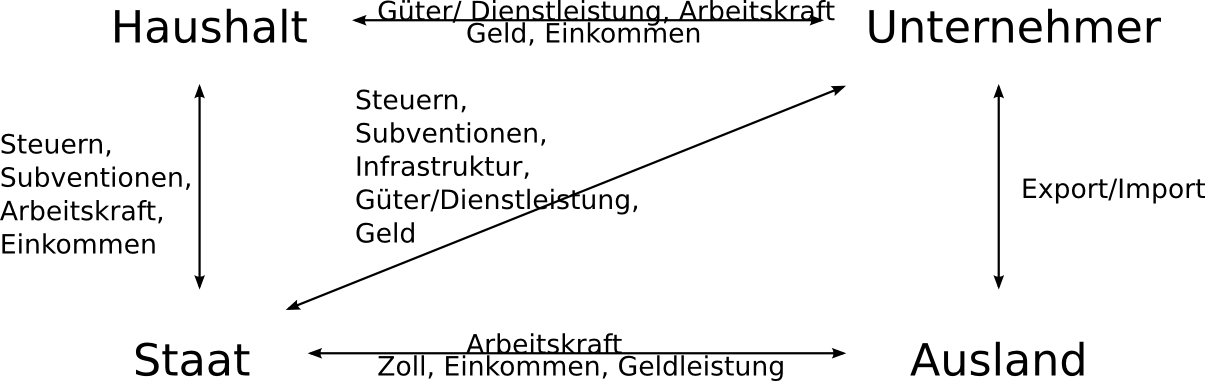
\includegraphics[scale=0.8]{image/image1.png}
\newline
\newline
\newline
\newline
Die Wirtschaftstätigkeit eines Landes wird zahlenmäßig erfasst, wobei verschiedene Ströme festgestellt werden. Zwischen den vier Wirtschaft Subjekten kommt es zu Transaktionen, Austausch von Gütern. Es gibt zwei gegenläufige Ströme:

\begin{itemize}
\item Realer Strom: Güter (Waren) und Dienstleistung
\item Monetärer Strom: Geld (Geldstrom)
\end{itemize}

Am Geldstrom wird das Volkseinkommen gemessen, am Güterstrom das Sozialprodukt. Das Sozialprodukt ist ein genereller Maßstab für die Wirtschaftskraft eines Landes. Je größer es ist, desto mehr kann im Allgemeinem verbraucht werden und desto größer ist der rechnerischer Wohlstand der Bevölkerung so fern dieser einigermaßen gleich verteilt ist.

\chapter{Güter}

Einteilung der Güter nach der Verfügbarkeit:

\begin{itemize}
\item öffentliche Güter (unbegrenzt vorhanden)
\item knappe Güter (Sachgüter, Dienstleistung, Rechte, Eigentumsrecht, ...)
\end{itemize}

Einteilung der Güter nach Verwendung:

\begin{itemize}
\item Konsumgüter
	\begin{itemize}
	\item Verbrauchsgüter (für einmaligen Gebrauch z.B. Nahrung, ...)
	\item Gebrauchsgüter (für mehrmaligen Gebrauch z.B. Auto, ...)
	\end{itemize}
\item Produktionsgüter (Güter mit den sich andere Güter herstellen lassen können)
\end{itemize}

\chapter{Produktionsfaktoren}

\section{Produktionsfaktoren}

\begin{itemize}
\item Boden
\item Arbeit
\item Wissen (Know-How)
\item Boden
\end{itemize}




\chapter{Taylorismus}

Wenn man einen komplexen Arbeitsprozess in möglichst viele kleinere Prozesse zerteilt, spricht man von Taylorismus. Zudem trennt man räumlich und personell die ausführende Arbeit mit der dispositiven Arbeit (Weisungsbefugnis).

\section{Vor- und Nachteile:}

\subsection{Vorteile:}

\begin{itemize}
\item Arbeiter benötigen nicht spezielles Wissen (billige Arbeitskräfte) oder lange Einarbeitungsphase
\item Arbeiter können leicht ersetzen werden
\item Transparenz in der Produktion und auch leichte Fehlersuche im Arbeitsprozess
\end{itemize}

\subsection{Nachteile:}

\begin{itemize}
\item Arbeiter langweilen sich, Monotonie $\rightarrow$ keine Motivation (kann zu Streiks führen)
\item körperliche Schäden $\rightarrow$ einseitige Belastung (z.B. Räder stemmen)
\item schlechtes Arbeitsklima, da es zu keiner Kommunikation zwischen den Arbeitern möglich ist
\item sinkende Lern- und Anpassungsmöglichkeiten an neue Aufgaben
\end{itemize}

\section{Andere Arbeitsformen}

\begin{itemize}
\item job rotation: Nach einem festen System werden regelmäßig die Arbeitsplätze getauscht. Die Struktur der Aufgaben wird nicht angerührt.
\item job enlargement: Zusätzliche Aufgaben werden zusammengeführt.
\item job enrichment: qualitative Ausweitung der Aufgaben, Eigenverantwortung
\item Team Arbeit (Projekt): große Motivation
\end{itemize}

\chapter{Wirtschaftssektoren}

\begin{itemize}
\item primärer Wirtschaftssektor: Urgewinnung
\item sekundärer Wirtschaftssektor: Produktion
\item tertiärer Wirtschaftssektor: Dienstleistung
\item quartärer Wirtschaftssektor: IT
\end{itemize}

\chapter{Arbeitslosigkeit}

\section{Definition}

Eine Person ist dann Arbeitslos, wenn die Person arbeitsfähig und arbeitswillig ist, sie schon einmal gearbeitet hat und nach Arbeit sucht.

\section{Arten der Arbeitslosigkeit}

\begin{itemize}
\item konjunkturelle Arbeitslosigkeit: die allgmeine Nachfrage nach Gütern und Dienstleistungen geht zurück $\rightarrow$ Arbeitskräfte werden entlassen $\rightarrow$ weitere Kaufkraft geht verloren.
\item strukturelle Arbeitslosigkeit: Verschiebung der Wirtschaftssektoren
\item friktionelle Arbeitlosigkeit: der Zeitraum ohne Arbeit den Arbeitsplätzen
\item saisoneale Arbeitslosigkeit: Seasonarbeit (z.B. Skifahren)
\item verdeckte Arbeitslosigkeit: betrifft Personen, die den Neueinstieg oder den Wiedereinstieg planen (z.B. Schüler, Frau nach Geburt)
\end{itemize}

\chapter{Konjunktur Theorie}

\begin{itemize}
\item John Majuard Kaynes (1883-1946)

In den 30er Jahren kam es Aufgrund der großen Weltwirtschaftskrise zu Massenarbeitslosigkeit. Kaynes empfahl der britischen Regierung, sich bei den Banken Geld zu leihen und damit Aufträge an die Industrie zu finanzieren. Die aufgenommenen Kredite könne man dann in der folgenden Boomphase (hohe Beschäftigung $\rightarrow$ reichliche Steuereinnahmen) wieder zurückzahlen.

\item Milton Friedman (1912-2006)

In den 60er Jahren feierte der Fiskalismus glanzvolle Erfolge. Viele glaubten, man könne die Wirtschaft nach belieben ''ankurbeln'' oder ''bremsen''. In den 70er kamen zweifel auf $\rightarrow$ wirtschaftliche Stagnation, hohe Arbeitslosigkeit bzw. Inflation. Friedman war der schärfste Kritiker des Kaynsianismus. Seine Meinung nach gehört der ganze ''Sozialklingbling'' (Kinder- oder Wohngeld) abgeschafft. Er leugnet zwar nicht die Möglichkeit von Arbeitslosigkeit, weil sich nicht alle Arbeitnehmer an veränderte Strukturen anpassen können oder wollen. Außerdem muss der Staat sich das zur Ausgaben finanzierende benötigte Geld auf dem Kapitalmarkt leihen $\rightarrow$ Zinsen steigen und private Investoren werden zurückgedrängt.
\end{itemize}

\chapter{Angebot und Nachfrage}

Nachfrage:
\newline
\newline

BILD

Die Nachfrage hängt ab von:

\begin{itemize}
\item Nutzen des Gutes
\item Einkommen $\rightarrow$ Kaufkraft
\item Qualität
\item Verfügbarkeit
\item Wertschätzung
\item Trend
\item Preis von Substitutionsgüter
\end{itemize}

Angebot:

BILD

Das Angebot hängt ab von:

\begin{itemize}
\item Produktionsbedienungen
\item Menge, die angeboten werden sollen
\item Kosten
\item Technologie
\end{itemize}

Beide Diagramme übereinander legen:
\newline
\newline

Markt Gleichgewicht.

\newpage

\section{Das Recht}

Es gibt Gesetze, die man vereinbart hat, um für Ordnung zu sorgen.

\begin{itemize}
\item \textbf{objektives Recht}: ist für die Gemeinschaft verbindliche Ordnung $\rightarrow$ Zusammenleben der Menschen $\rightarrow$ Durchsetzung durch Zwang; ist bei allen Menschen gleich
\item \textbf{subjektives Recht}: ist das Recht das jedem Einzelnen von uns zusteht z.B. Eigentumsrecht, Erbrecht, usw.; Eigentumsrecht und Erbrecht ist individuell
\end{itemize}

Öffentliches Recht  $\rightarrow$ Beziehung zwischen Einzelperson und Staat
\newline
Privates Recht $\rightarrow$ Beziehung zwischen Privatpersonen

\subsection{Gruppenarbeit}

\subsubsection{Stufenbau der Rechtsordnung}

\begin{itemize}
\item EU
\item Verfassung
\item Gesetze z.B. Schulpflicht (Leistungsbeurteilung, Recht auf Benotung, Pflicht der Lehrer)

	\begin{itemize}
	\item Bundesgesetz z.B. Höchstgeschwindigkeit (ABGB; Allgemeine Bürgerliches Gesetz Buch; Grundlagen aller Gesetzte)
	\item Landesgesetz z.B. Jugendschutzgesetz
	\end{itemize}

\item Verordnungen: sind dazu da die Gesetze in die Praxis umzusetzen z.B. wie der Lehrer unterrichten muss, ob er Schularbeiten machen darf oder nicht
\item Bescheid: z.B. positives Bescheid (Baubescheid, ...); negative Bescheid (Führerschein Entzug, ...)
\item Urteile
\item Strafen
\end{itemize}

\subsubsection{Grundprinzipien der Verfassung}

\begin{itemize}
\item Grundprinzipien:

	\begin{itemize}
	\item \textbf{demokratische Prinzip}
	
			\begin{itemize}
			\item indirekte
			\item direkte
			\item Volksbefragung (Ergebnis hat keine Auswirkung)
			\item Volksbegehren (braucht es mindesten 100.000 Stimmen in Form von Unterschriften, dann geht es in den National Rat)
			\item Volksabstimmung (Änderung der Verfassung) z.B. Österreich beitritt zur EU
			
			\item Wahlrecht
				\begin{itemize}
				\item aktives Wahlrecht (16 Jahren)
				\item passives Wahlrecht (19 Jahren)
				\end{itemize}		
			\end{itemize}				
	
	\item \textbf{republikanisches Prinzip}
	
		\begin{itemize}
		\item das Staatsoberhaupt ist der Bundespräsidenten (kann einmal wiedergewählt werden; maximal 12 Jahre)
		\end{itemize}			
	\item \textbf{bundesstaatliche Prinzip}: Gesetzgebung und vollziehen sind zwischen Bund und Land aufgeteilt $\rightarrow$ Kompetenzverteilung, wobei die wichtigsten Staatsaufgaben den Bund zugewiesen werden z.B. die Finanzen.
	\item \textbf{liberales Prinzip}:die staatliche Verwaltung darf nur auf Grundlagen der Gesetze ausgeübt werden
	\item \textbf{reststaatliches Prinzip}: welchen Aufbau haben wir in Österreich? Legislative, Exekutive, Judikative. Gewaltentrennung!
	\end{itemize}
\end{itemize}

\begin{itemize}
\item Zwingendes Recht $\rightarrow$ Recht/ Pflicht das jeder machen muss z.B. Schulpflicht

\item Nachgiebiges Recht $\rightarrow$ Gesetzliche Vorschrift, die durch Parteienänderung abgeändert werden.

\end{itemize}

Personen:

\begin{itemize}
\item natürlichen Personen
\item juristischen Personen $\rightarrow$ Zusammenschluss von mehreren Personen, die nach außen hin eine Einheit bilden und ein Ziel verfolgen z.B. Kapitalgesellschaften (AG und Gesmbh), Vereine, Gebietskörperschaften (Bund, Land, Gemeinde). 
\end{itemize}

Über welche Fähigkeiten verfügen diese Personen? | Rechtsfähigkeit = Trägen von Rechte und Pflichten zu sein. Die sogenannte Handlungsfähigkeit ist die Fähigkeit der Handlungen $\rightarrow$ das man für sich selber Verantwortlich ist (hängt ab vom geistlichen Zustand ab).
\newline
\newline
Unterteilung der Handlungsfähigkeit

\begin{itemize}
\item Geschäftsfähigkeit | Abhängig vom Alter und der geistlichen Reife
\item Deliktsfähigkeit  | Abhängig vom Alter und der geistlichen Reife (ist man am 14ten Geburtstag); man wir für seine Taten zur Verwantwortung gezogen.
\end{itemize}

Altersstufen:

\begin{enumerate}
\item 0 bis 7 ... Kinder (bis zum Vollenden siebten Lebensjahr) (beschränkt Geschäftsfähig)
\item 7 bis 14 ... unmündige Minderjährigen (beschränkt Geschäftsfähig; sie können sehr Wohl Rechte erwerben, ein zu ihrem Vorteil gemachtes Versprechen)
\item 14 bis 18 ... mündige Minderjährigen (ihnen räumt das Gesetzt eine weitergehende Geschäftsfähigkeit ein, d.h. sie können sich selbständig Vertraglich zu Dienstleistung verpflichten, Ausnahme: Lehrverträge; der Mündige dürfen über ihr Einkommen frei verfügen, sofern die Befriedigung der Lebensbedürfnisse nicht gefährdet wird)
\item größer 18 ... volljährig
\end{enumerate}

1 bis 2 sind nur teilweise Geschäftsfähig.

\section{Gesetzliche Vertretung}

Personen, die nicht handlungsfähig sind, bedürfen einen gesetzlichen Vertreter. Falls die Eltern nicht vorhanden sind, ist der gesetzlich Vertreter der Vormund (=Opa,Oma bzw. Personen zu denen ein nahes Verhältnis besteht). Bei mangelten Geisteskraft $\rightarrow$ Sachwalter; vertritt Personen die ihre Angelegenheiten nicht ohne Gefahr eines Nachteils für sich selbst besorgen können. 
\begin{itemize}
\item Bei einzelnen Angelegenheiten (z.B. geistige Behinderung und Testament)
\item bestimmter Bereich (finanzieller Bereich) (z.B. alle Angelegenheiten einer geistlich behinderten Personen)
\end{itemize}

Sachwalter:

\begin{itemize}
\item Familienangehörige
\item bei rechtlichen Angelegenheiten (Interessenkonflikten = dann übernimmt ein Rechtsanwalt)
\end{itemize}

\section{Sachrecht}



\end{document}
